\documentclass[8pt,aspectratio=169,xcolor=dvipsnames]{beamer} % use handout option for handouts

%\usepackage{pgfpages}
%\pgfpagesuselayout{2 on 1}[a4paper,border shrink=5mm]

\usepackage[utf8]{inputenc}
\usepackage{colortbl}
\usepackage{multimedia}

\usetheme{default}
\usecolortheme{seagull}

\usepackage[T1]{fontenc}
\usepackage[light]{roboto} 
\usefonttheme[onlymath]{serif}

\usepackage{mwe} % provides images used in this example

\usepackage{pgf,tikz}
\usetikzlibrary{shapes.geometric, arrows}

\usepackage{pgfplots}
%\usepgfplotslibrary{external}
%\tikzexternalize

%%%%%%%%%%%%%%%%%%%%%%%%%%%%%%%%%%%%%%%%%%%%%%%%%%%%%%%%%%%%%%%%%%%%%%%%%%%%%%%%%%%%%%%

\setbeamertemplate{frametitle}{\color{black}\bfseries\vskip16pt\insertframetitle}
\setbeamertemplate{footline}[frame number]

\linespread{1.25}

\definecolor{ImperialRed}{HTML}{e63946}
\definecolor{HoneyDew}{HTML}{f2efef}
\definecolor{PowderBlue}{HTML}{A8DADC}
\definecolor{CeladonBlue}{HTML}{457B9D}
\definecolor{PrussianBlue}{HTML}{1D3557}


\setbeamercolor{block title}{bg=PrussianBlue,fg=white}
\setbeamercolor{block title example}{bg=CeladonBlue,fg=white}
\setbeamercolor{block title alerted}{bg=ImperialRed,fg=white}

\setbeamercolor{block body}{bg=HoneyDew,fg=black}
\setbeamercolor{block body example}{bg=HoneyDew,fg=black}
\setbeamercolor{block body alerted}{bg=HoneyDew,fg=black}

\setbeamerfont{block title}{size=\normalsize}
\setbeamerfont{block body}{size=\normalsize}
\setbeamerfont{block title example}{size=\normalsize}
\setbeamerfont{block body alerted}{size=\normalsize}
\setbeamerfont{block body example}{size=\normalsize}

\setbeamercolor{alerted text}{fg=ImperialRed}

% table definitions
\newcolumntype{a}{>{\columncolor{ImperialRed!70}}c}
% Change horizontal spacing
\setlength{\tabcolsep}{20pt}
% Change vertical spacing
\renewcommand{\arraystretch}{1.5}


% tikz definitions
\tikzset{
  invisible/.style={opacity=0},
  visible on/.style={alt={#1{}{invisible}}},
  alt/.code args={<#1>#2#3}{%
    \alt<#1>{\pgfkeysalso{#2}}{\pgfkeysalso{#3}} % \pgfkeysalso doesn't change the path
  },
}
\tikzstyle{startstop} = [rectangle, rounded corners, minimum width=2cm, minimum height=1cm,text centered, draw=black, fill=ImperialRed, text = white]
\tikzstyle{io} = [trapezium, trapezium left angle=70, trapezium right angle=110, minimum width=2cm, minimum height=1cm, text centered, draw=black, fill=CeladonBlue, text = white]
\tikzstyle{process} = [rectangle, minimum width=2cm, minimum height=1cm, text centered, draw=black, fill=HoneyDew, text width = 2cm]
\tikzstyle{decision} = [diamond, minimum width=2cm, minimum height=1cm, text centered, draw=black, fill=PowderBlue]
\tikzstyle{arrow} = [thick,->,>=stealth]




%------------------------------------------------------------
%This block of code defines the information to appear in the
%Title page
\title[About Beamer] %optional
{\textbf{About the Beamer class in presentation making}}

\subtitle{A short story}

\author[Schramm, Georg] % (optional)
{Georg Schramm\inst{1}}

\institute[KUL] % (optional)
{
  \inst{1}%
  Department of Imaging and Pathology\\
  KU Leuven
}

\date[VLC 2021] % (optional)
{Very Large Conference, April 2021}

%\logo{\includegraphics[height=1cm]{overleaf-logo}}

%End of title page configuration block
%------------------------------------------------------------



%------------------------------------------------------------
%The next block of commands puts the table of contents at the 
%beginning of each section and highlights the current section:

\AtBeginSection[]
{
  \begin{frame}
    \frametitle{Table of Contents}
    \tableofcontents[currentsection]
  \end{frame}
}
%------------------------------------------------------------


\begin{document}

%The next statement creates the title page.
\frame{\titlepage}


%---------------------------------------------------------
%This block of code is for the table of contents after
%the title page
\begin{frame}
\frametitle{Table of Contents}
\tableofcontents
\end{frame}
%---------------------------------------------------------


\section{First section}

%---------------------------------------------------------
%Changing visivility of the text
\begin{frame}
\frametitle{Sample frame title}
This is a text in second frame. For the sake of showing an example.

\begin{itemize}
    \item<1-> Text visible on slide 1
    \item<2-> Text visible on slide 2
    \item<3>  Text visible on slide 3
    \item<4-> Text visible on slide 4
\end{itemize}
\end{frame}

%---------------------------------------------------------

\begin{frame}
\frametitle{Tikz flow chart}

\begin{center}
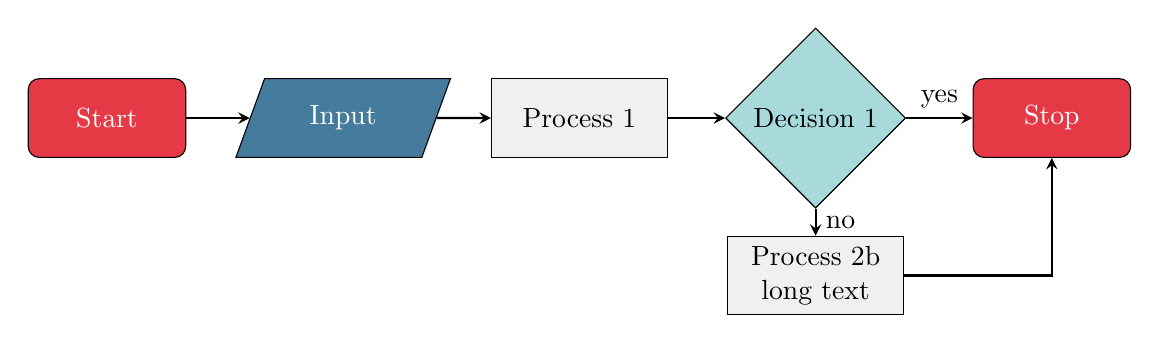
\begin{tikzpicture}[node distance=3cm]
\node (start) [startstop] {Start};
\node (in1) [io, right of=start, visible on = <2->] {Input};
\node (pro1) [process, right of=in1, visible on = <3->] {Process 1};
\node (dec1) [decision, right of=pro1, visible on = <4->] {Decision 1};
\node (pro2b) [process, below of=dec1, yshift = 1cm, visible on = <6->] {Process 2b long text};
\node (stop) [startstop, right of=dec1, visible on = <5->]{Stop};

\draw [arrow, visible on = <2->] (start) -- (in1);
\draw [arrow, visible on = <3->] (in1)   -- (pro1);
\draw [arrow, visible on = <4->] (pro1)  -- (dec1);
\draw [arrow, visible on = <6->] (dec1)  -- node[anchor=west]  {no} (pro2b);
\draw [arrow, visible on = <5->] (dec1)  -- node[anchor=south] {yes} (stop);
\draw [arrow, visible on = <6->] (pro2b) -| (stop);
\end{tikzpicture}
\end{center}

\end{frame}

%---------------------------------------------------------
\begin{frame}{Colored tables}
\centering
\begin{tabular}{lrara}
\hline
\rowcolor{PowderBlue}
    \textbf{variables} & \multicolumn{4}{c}{\textbf{data}}\\ \hline
    var 1 & 1 & 2 & 3 & 4 \\ \hline
    var 2 & 1 & 2 & 3 & 4 \\ \hline
    var 3 & 1 & 2 & 3 & 4 \\ \hline
\end{tabular}
\end{frame}
%---------------------------------------------------------

\section{Second section}

%---------------------------------------------------------
%Highlighting text
\begin{frame}
\frametitle{Sample frame title}

In this slide, some important text will be
\alert{highlighted} because it's important.
Please, don't abuse it.

\begin{block}{Remark}
Sample text
\end{block}

\begin{alertblock}{Important theorem}
Sample text in red box
\end{alertblock}

\begin{examples}
Sample text in green box. The title of the block is ``Examples".
\end{examples}
\end{frame}
%---------------------------------------------------------


%---------------------------------------------------------
%Two columns
\begin{frame}
\frametitle{Two-column slide}

\begin{columns}

\column{0.4\textwidth}
This is a text in first column.
$$E=\int f(x) dx$$
\begin{itemize}
\item First item
\item Second item
\end{itemize}

\column{0.5\textwidth}

%\begin{figure}
\begin{center}
\resizebox{0.95\columnwidth}{!} {%
  \definecolor{zzttqq}{rgb}{0.6,0.2,0}
\definecolor{xdxdff}{rgb}{0.49,0.49,1}
\definecolor{qqqqff}{rgb}{0,0,1}
\definecolor{cqcqcq}{rgb}{0.75,0.75,0.75}
\begin{tikzpicture}[line cap=round,line join=round,>=triangle 45,x=1.0cm,y=1.0cm]
\draw [color=cqcqcq,dash pattern=on 1pt off 1pt, xstep=2.0cm,ystep=2.0cm] (-2,-2) grid (7,7);
\draw[->,color=black] (-2,0) -- (7,0);
\foreach \x in {-2,2,4,6}
\draw[shift={(\x,0)},color=black] (0pt,2pt) -- (0pt,-2pt) node[below] {\footnotesize $\x$};
\draw[->,color=black] (0,-2) -- (0,7);
\foreach \y in {-2,2,4,6}
\draw[shift={(0,\y)},color=black] (2pt,0pt) -- (-2pt,0pt) node[left] {\footnotesize $\y$};
\draw[color=black] (0pt,-10pt) node[right] {\footnotesize $0$};
\clip(-2,-2) rectangle (7,7);
\fill[color=zzttqq,fill=zzttqq,fill opacity=0.1] (0.56,2.48) -- (0.5,0.94) -- (2.64,0.58) -- (2.3,1.76) -- (1.68,2.62) -- cycle;
\draw [domain=-2:7] plot(\x,{(--24-4*\x)/6});
\draw [color=zzttqq] (0.56,2.48)-- (0.5,0.94);
\draw [color=zzttqq] (0.5,0.94)-- (2.64,0.58);
\draw [color=zzttqq] (2.64,0.58)-- (2.3,1.76);
\draw [color=zzttqq] (2.3,1.76)-- (1.68,2.62);
\draw [color=zzttqq] (1.68,2.62)-- (0.56,2.48);
\draw(0,4) circle (1cm);
\begin{scriptsize}
\fill [color=qqqqff] (0,4) circle (1.5pt);
\draw[color=qqqqff] (0.16,4.26) node {$A$};
\fill [color=xdxdff] (6,0) circle (1.5pt);
\draw[color=xdxdff] (6.16,0.26) node {$B$};
\fill [color=qqqqff] (0.56,2.48) circle (1.5pt);
\draw[color=qqqqff] (0.72,2.74) node {$C$};
\fill [color=qqqqff] (0.5,0.94) circle (1.5pt);
\draw[color=qqqqff] (0.66,1.2) node {$D$};
\fill [color=qqqqff] (2.64,0.58) circle (1.5pt);
\draw[color=qqqqff] (2.8,0.84) node {$E$};
\fill [color=qqqqff] (2.3,1.76) circle (1.5pt);
\draw[color=qqqqff] (2.44,2.02) node {$F$};
\fill [color=qqqqff] (1.68,2.62) circle (1.5pt);
\draw[color=qqqqff] (1.84,2.88) node {$G$};
\end{scriptsize}
\end{tikzpicture}

}
\end{center}
%\caption{Foo bar}
%\end{figure}

\end{columns}
\end{frame}
%---------------------------------------------------------

%---------------------------------------------------------
%Two columns
\begin{frame}
\frametitle{Math}

\begin{equation}
    \lambda^+ = \lambda \sum_i \frac{y_i}{\bar{y}_i}
\end{equation}

\end{frame}
%---------------------------------------------------------

\begin{frame}[t]
\frametitle{Test}

\begin{block}<1->{Correction method}
  \begin{itemize}
    \item<2-> Simulate
    \item<5-> Assign
  \end{itemize}
\end{block}

\begin{onlyenv}<3-6>
  \begin{center}
    \includegraphics<3>[scale=0.4]{image-a}
    \includegraphics<4>[scale=0.4]{image-b}
    \includegraphics<6>[scale=0.4]{image-c}
  \end{center}
\end{onlyenv}

\begin{onlyenv}<7->
  \begin{block}<7->{Scores}
    \begin{itemize}
      \item<8-> PSNR
      \item<9-> MSE
    \end{itemize}
  \end{block}
\end{onlyenv}

\begin{center}
  \includegraphics<10>[scale=0.2]{image-a}
  \includegraphics<10>[scale=0.2]{image-b}
\end{center}
\end{frame}  

\end{document}
